\chapter{TINJAUAN PUSTAKA}
\label{chap:tinjauanpustaka}

% Ubah bagian-bagian berikut dengan isi dari tinjauan pustaka
\section{Penelitian Terdahulu}
\label{sec:penelitianterdahulu}

Pada penelitian yang telah dilakukan oleh Reza Putra Pradana bertajuk \emph{Sistem Transaksi Antar Player Pada Game Multiplayer Wisata Bromo Menggunakan Blockchain} dikemukakan bahwa transaksi digital bisa menggunakan \emph{Ethereum} dengan harga per transaksi Rp.471 dengan kecepatan antara 3 - 30 detik \cite{pradana2020}. Pada penelitian yang dilakukan oleh Reza Putra Pradana, dilakukan penelitian dan penjelasan mengenai penggunaan \emph{Blockchain Ethereum} untuk sistem pembayaran di dalam game yang dia buat. Dalam game tersebut dibuat menggunakan Game Engine Unity dan sistem pembayaran yaitu Ethereum. Dengan menggunakan Unity tersebut dibuat sistem game role play gaming yang mana pengguna berperan sebagai pengunjung/wisatawan yang mengunjungi daerah Gunung Bromo. Dalam kawasan Gunung Bromo tersebut terdapat kegiatan yang bisa dilakukan di dalam kawasan mulai dari masuk ke kawasan sekitar kawah gunung, membeli makan, membeli tiket, hingga menyewa kendaraan. Semua interaksi di dalam kawasan Gunung Bromo dilakukan melalui interaksi NPC dan menggunakan mata uang Ether. Untuk pengujian sistem transaksi menggunakan \emph{provider} internet mobile Indonesia, dan mendapatkan hasil performa latensi yang diterima antara perangkat pengunjung dengan perangkat NPC berkisar antara 61ms - 144ms. Angka ini tergolong memiliki performa cukup untuk digunakan sehari hari. Kemudian performa sistem Ethereum yang digunakan menelan biaya berkisar antara Rp300.000,- hingga Rp3.000.000,- per bulan dengan rincian Rp300,- hingga Rp3.000,- per transaksi x 1000 transaksi per bulan.

\section{Validasi}
\label{sec:validasi}

Melansir dari KBBI daring, validasi adalah sebuah kegiatan untuk melakukan pengujian kebenaran atas sesuatu. Dalam lingkup Ethereum validasi adalah serangkaian kegiatan untuk menguji kebenaran suatu transaksi yang akan dilakukan. Pengujian kebenaran data suatu transaksi dilakukan agar tidak terjadi kesalahan data pada suatu transaksi. Kesalahan yang dimaksud bisa terjadi dari luar sistem maupun dalam sistem. Apabila terjadi kesalahan data bisa membaut suatu transaksi tidak terjadi. Kesalahan data internal yang biasa terjadi adalah kesalahan penyediaan dan perhitungan gas. Sedangkan dari luar sistem bisa saja ada upaya interupsi transaksi. Interupsi interaksi ini bisa berupa serangan 51\% / 51\% attack di suatu sistem Ethereum. Dalam arsitektur Ethereum, proses pengujian kebenaran data yang dikirim (validasi) menggunakan sebuah  kesepakaran yaitu kesepakatan yang biasa disebut konsensus. Konsensus ini memungkinkan validasi sebuah data menggunakan tenaga komputer lainnya yang telah tergabung dengan berbagai syarat dari Ethereum itu sendiri.

\section{Kriptografi}
\label{sec:kriptografi}

Kriptografi adalah sebuah cara untuk mengamankan informasi yang dikirimkan oleh pengirim kepada penerima. Kriptografi memiliki peran dalam keamanan siber terutama dalam kerahasiaan inform si yang dikirim. Kerahasiaan informasi ini menjamin data dikirimkan tidak diubah selama dalam pengiriman dari pengirim ke penerima \cite{stallings1999cryptography}. Kriptografi mempunyai tujuang sebagai metode untuk mengenkripsi dan mendekripsi informasi yang dikirim dengan beberapa standar. Dalam Ethereum, kriptografi digunakan sebagai standar pembuatan blok baru yang telah divalidasi.  

\subsection{Fungsi Hash}
\label{subsec:hashfunction}

Fungsi hash adalah sebuah standar kriptografi yang mengenkripsi informasi yang dikirimkan dengan menggunakan matematika untuk memadatkan informasi yang dikirim dan menjadikannya satu potong informasi tetap yang utuh \cite{stallings1999cryptography}. Dalam praktiknya fungsi hash akan memproses informasi yang sangat banyak yang akan dikirim kemudian akan mengeluarkan nilai hash yang mempunyai jumlah tetap. Ini artinya fungsi hash memangkas jumlah data yang dikirim setelah di enkripsi dan selanjutnya dikirim dan di-dekripsikan oleh penerima. Apabila jumlah data yang dikirimkan sejulah 512bit maka apabila dilakukan fungsi hash akan tereduksi menjadi sekitar 160bit. Hasil dari fungsi hash ini akan terdiri atas kombinasi angka, huruf, dan simbol. Sedikit perbedaan informasi yang dienkripsi fungsi hash, maka hasil yang didapatkan akan menjadi berbeda sama sekali. Namun dalam praktiknya fungsi hash ini memerlukan banyak komputasi dan data yang bisa diproses pun dipecah menjadi beberapa bagian kecil.Karena hal ini fungsi hash digunakan di beberapa aplikasi saja. Dan dalam upaya menaikkan performa ini tercipta suatu fungsi hash yaitu SHA (\emph{Secure Hash Algorithm}).

\subsection{SHA (\emph{Secure Hash Algorithm})}
\label{subsec:sha}

SHA adalah salah satu jenih fungsi hash yang saat ini banyak digunakan sebagai tanda unik untuk mengetahui bahwa integritas suatu informasi. Dalam upaya untuk memecahkan informasi yang telah melalui fungsi hash, perlu dilakukan 'tenaga paksa' yang mana pada konteksnya berupaya mencocokkan suatu hasil output dengan input satu per satu dan dicoba secara berulang \cite{stallings1999cryptography}. SHA ditemukan oleh NIST (\emph{National Institute of Standards and Technology}) yang pada awalnya dapat mereduksi 512 bit menjadi 160 bit. Kemudian SHA pertama (SHA-0) terus dikembangkan dan terjadi beberapa iterasi hingga menjadi SHA-2 yang saat ini banyak digunakan.
\\
\begin{figure}
	\centering
	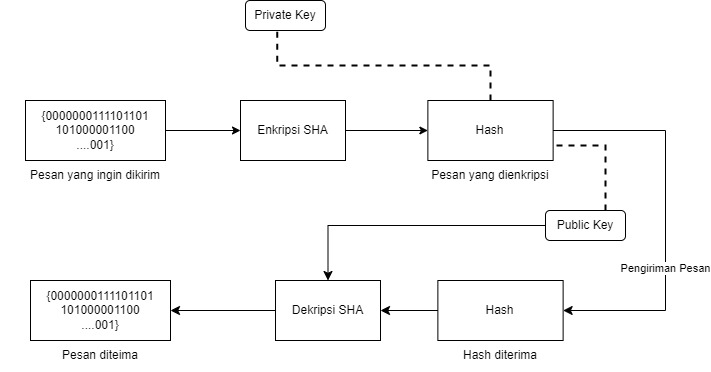
\includegraphics[scale=0.5]{gambar/sha.jpg}
	\caption{Ilustrasi SHA}
	\label{fig:shaillustrated}
\end{figure}
\\
Dalam praktiknya, SHA melakukan enkripsi dengan mengubah pesan yang ada menjadi angka dan huruf acak. Dalam proses enkripsinya akan diciptakan dua buah rangkaian kunci yaitu kunci publik dan kunci privat. Setelah enkripsi pesan selesai, ukuran pesan tereduksi dan menghasilkan kunci publik dan kunci privat. Pada kunci privat akan menjadi kunci yang krusial dalam menandakan pesan yang kita kirim. Kunci privat digunakan sebagai 'tanda tangan' kita dalam pesan yang terenkripsi. Kemudian kunci public bisa diberikan kepada penerima pesan sebagai autentikasi pesan yang kita enkripsi di awal adalah pesan sama yang telah diterima. Sedangkan kunci privat digunakan sebagai 'bon' bahwa kita telah melakukan SHA.Selanjutnya di sisi penerima pesan didekripsi sambil dicocokkan dengan kunci publik yang diberikan. Apabila kunci publik dengan pesan tidak cocok, maka pesan yang terenkripsi telah berubah dalam pengiriman. Apabila dalam proses enkripsi pesan yang dienkripsi mencapai limit,otomatis akan dilakukan iterasi enkripsi dengan sebagian pesan yang telah dienkripsi hingga semua pesan telah dienkripsi. Dan apabila dalam proses enkripsi panjang pesan tidak mencapai jumlah bit yang dienkripsi maka akan dilakukan padding dengan mengisi pesan yang kosong dengan 0 dan kemudian mengisi bit terakhir dengan panjang pesan terakhir yang belum dienkripsi \cite{stallings1999cryptography}.
\\
Dalam SHA tidak bisa dilakukan enkripsi dan dekripsi secara universal. Artinya data suatu SHA yang dienkripsi tidak bisa dilacak dari satu database ke database lainnya. Karena dalam enkripsi SHA, hash yang telah tersimpan hanya satu dan unik. Maka apabila suatu hash dari SHA tidak bisa didekripsikan dengan mesin SHA yang berbeda. 

\section{\emph{Smart Contract}}
\label{sec:smartcontract}

Smart Contract adalah sebuah program yang bisa berjalan dalam suatu Blockchain yang dipilih. Dalam Blockchain, smart contract menjadi tempat untuk menampung data dan fungsi. Untuk menjalankan smart contract diperlukan beberapa variabel dan memenuhi syarat fungsi itu sendiri untuk berjalan misalnya "if.. else/while" dan sejenisnya. Namun, dalam smart contract sendiri memiliki kekurangan dalam pengembangannya. Dikarenakan berjalan pada Blockchain, smart contract-nya setelah dikirim ke Blockchain tidak bisa dimodifikasi sedikit pun.
\\
Karena smart contract adalah suatu pusat dari kegiatan teknis sebuah Blokchain yang terus berjalan di masing-masing blok, smart contract ini menjadi inti dari keseluruhan Blockchain yang mana di dalamnya terdapat beberapa fungsi fungsi yang bisa dijalankan setelah mendapatkan input yang tepat. Dalam smart contract sendiri, ada susunan elemen yang harus ada seperti inisiasi compiler yang digunakan, alamat dan constructor, pointer memory, hingga fungsi yang ingin kita implementasikan ke dalam smart contract. Apabila beberapa elemen ini tidak hadir di dalam smart contract kita otomatis smart contract bisa tidak berjalan.
\\
Untuk menjalankan sebuah smart contract di Blockchain karena tidak tersentral,maka memerlukan sebuah pertukaran usaha membuat blok antara pembuat blok dan yang meminta blok dibuat dari suatu jaringan Blockchain. Maka smart contract memerlukan gas untuk membuat blok baru.

\subsection{Gas}
\label{subsec:gas}

Gas adalah sebuah biaya yang diperlukan untuk melakukan sebuah kegiatan pembuatan blok dalam Blockchain via smart contract. Sebuah gas dapat menjadi sebuah biaya untuk melakukan fungsi di dalam smart contract yang memerlukan validasi blok. Gas ini diperlukan sebagai biaya melakukan transaksi yang bisa diatur jumlah yang bisa disediakan dan harga satuan dari gas tersebut. Pengguna bisa melakukan pembatasan gas yang bisa dipakai dan harga gas yang bisa dipergunakan per satu. Gas tersebut akan digunakan untuk membiayai transaksi yang dilakukan, dan jumlah gas bisa bertambah apabila gas tidak mencukupi. Jumlah gas yang akan terpakai akan mengambil sejumlah cryptocurrencies yang kita miliki dalam akun blockchain. Maka sebelum dilakukan transaksi, jumlah gas yang akan terpakai ditambahkan otomatis ke transaksi yang dilakukan.

\section{\emph{Blockchain}}
\label{sec:blockchain}

\emph{Blockchain} adalah sebuah jaringan \emph{peer-to-peer} yang dienkripsi oleh kriptografi SHA untuk mengirimkan dan menyimpan data, hosting aplikasi, hingga pertukaran value yang merepresentasikan mata uang fisik dan didistribusikan secara desentralisasi \cite{bookethsol}.Popularitas \emph{Blockchain} mulai meningkat pada tahun 2013 yang ditandai dengan kenaikan nilai \emph{Bitcoin} yang merupakan mata uang kripto populer pertama di dunia. Semenjak saat itu \emph{Blockchain} semakin dilirik karena \emph{Cryptocurrencies} yang terkandung di dalamnya. \emph{Blockchain} bisa diibaratkan sebagai buku kas yang dimiliki dan bisa diakses oleh semua orang yang tergabung dalam satu jaringan \cite{8701371}.Dalam buku publik tersebut terdapat sejumlah hash yang tersimpan dengan berbagai macam informasi yang telah dienkripsi. Informasi ini bebas diakses oleh siapapun yang tergabung dalam jaringan \emph{Blockchain}.Dan apabila dilakukan suatu inisiasi perubahan data dalam suatu blok otomatik akan ada perubahan kunci publik dan kunci privat yang dimiliki.

\begin{figure}[htp]
  \centering
  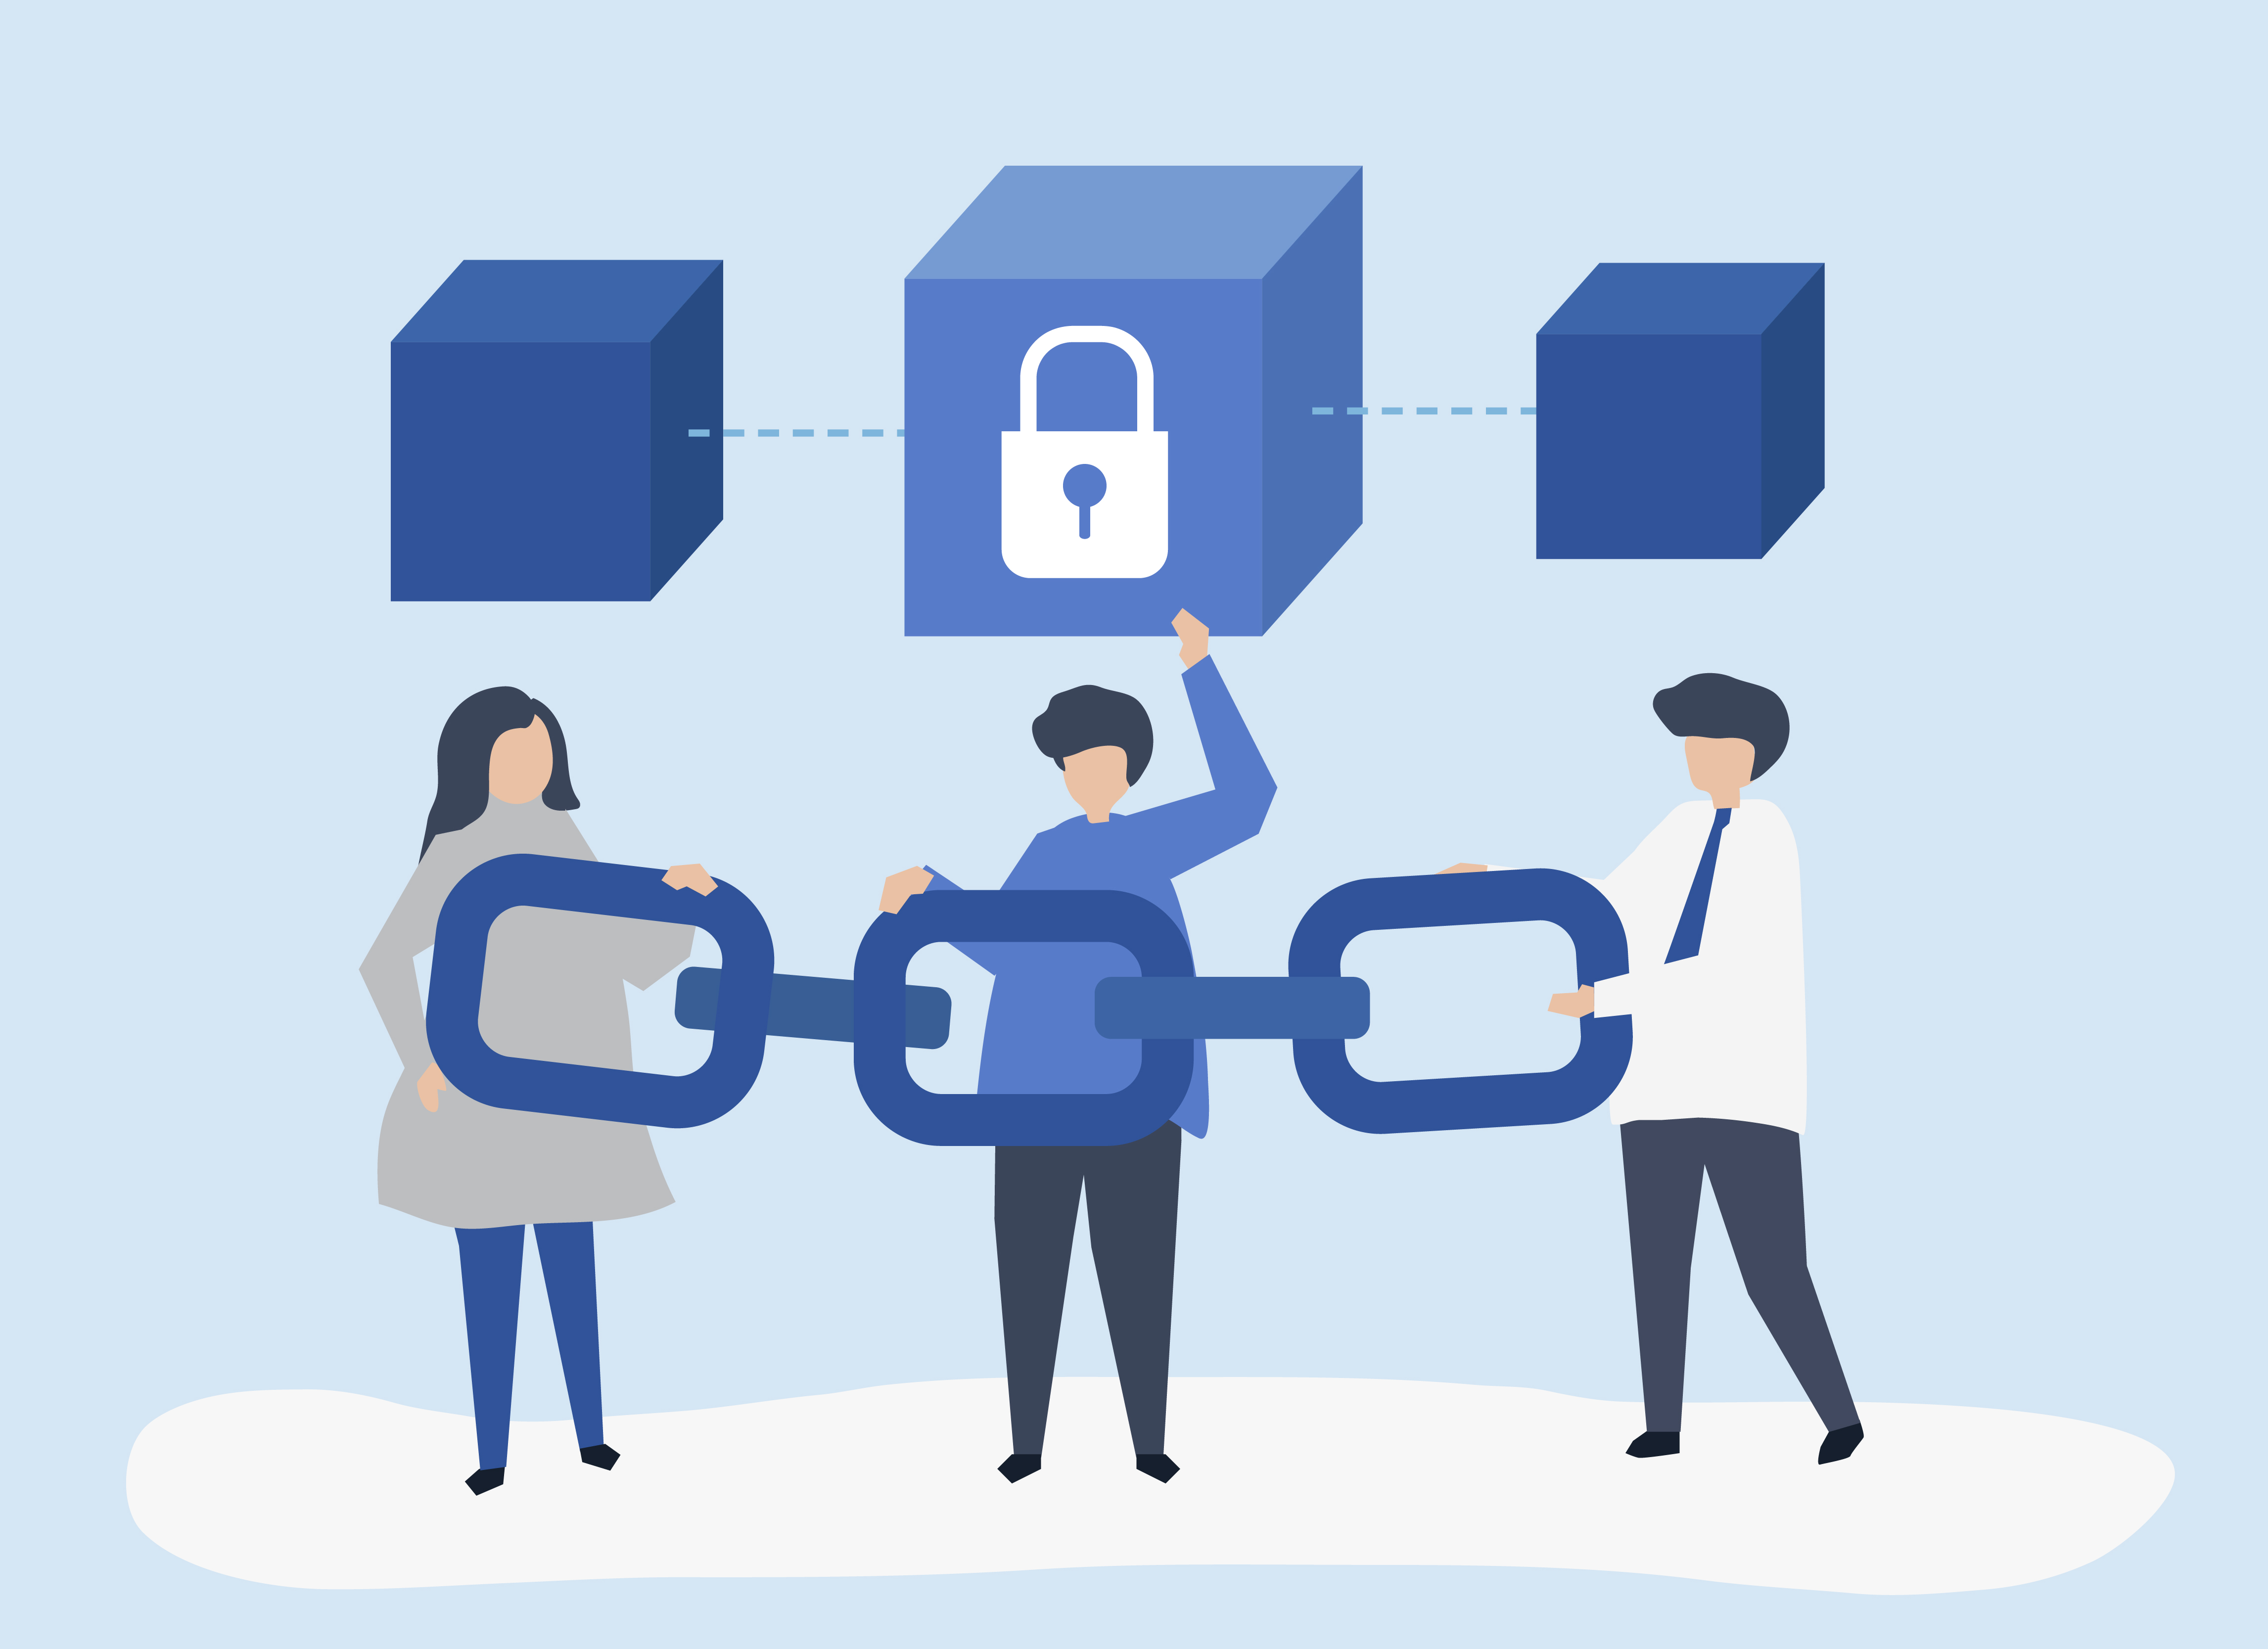
\includegraphics[scale=0.2]{gambar/blockchain-illustrated.jpg}
  \caption{Ilustrasi \emph{Blockchain}}
  \label{fig:blockchainillustrated}
\end{figure}

Untuk dapat dikatakan sebuah \emph{blockchain}, sebuah sistem harus memenuhi beberapa syarat yang dapat ditemui hanya di \emph{blockchain}. Syarat tersebut adalah :

\begin{itemize}
\item{\emph{Immutability}}\\Adalah suatu syarat bahwa data apapun yang telah termuat di dalam suatu blok harus tidak bisa diubah oleh siapapun dalam blockchain tersebut. Yang dimaksud di sini adalah sistem tersebut mempunyai segelintir aturan yang ditetapkan agar data yang telah termuat di suatu blok tidak diubah semena-mena.
\item{Terdistribusi}\\Data yang ada dalam blokchain harus didistribusikan ke seluruh pengguna yang terhubung baik melalui node maupun melalui langsung. Blok data yang terdistribusi harus dimiliki oleh semua penggna.
\item{Tranparan}\\Data yang dikirim pun tidak boleh melalui proses selektif sistem. Blok data yang dikirim oleh blockchain harus seadanya dan tanpa ada modifikasi.
\item{Terdesentralisasi}\\Terdesentralisasi artinya tidak ada pihak utama dalam suatu blockchain yang mengambil keputusan blockchain tersebut. Alih - alih node yang telah terhubung harus membiarkan hal ini tetap terjadi.
\item{Aman}\\Tentu untuk menjamin \emph{Immutability} diperlukan pengamanan yang tepat untuk menjalankan blockchain secara paralel dan tidak terinterupsi.
\item{Konsensus}\\Konsensus adalah sebuah mekanisme kesepakatan yang digunakan oleh blockchain untuk menjaga seluruh sistem tetap adil untuk semua orang. Tentu konsensus ini juga diperlukan agar sistem bisa berjalan cepat dan efektif dalam membuat blok baru.
\end{itemize}

\emph{Blockchain} memiliki banyak konfigurasi mulai dari jenis kriptografi yang digunakan, konsensus yang digunakan, hingga pengaplikasian yang digunakan. Salah satu pembeda \emph{Blockchain} yang cukup terlihat adalah jenis konsensus yang digunakan. Konsensus adalah proses pemufakatan yang dilakukan oleh pengguna dalam suatu jaringan \emph{Blockchain}. Saat ini banyak jenis konsesus yang digunakan mulai dari \emph{Proof of Work, Proof of Authority}, hingga \emph{Proof of Stake}. Dalam sistem sebuah Blockchain terdapat berbagai konfigurasi yang digunakan. Berfokus pada fitur dan keunggulan masing masing. Konfigurasi tersebut berupa jenis konsensus yang dipakai, enkripsi yang digunakan, smart contract yang bisa digunakan, hingga dokumentasi untuk forking blockchain tersebut.
\\ \\ \\
Dalam susunan suatu blok dari blockhain terdapat standar isi dari suatu blok yang telah terbuat. Dalam satu blok yang telah terbuat, terdapat block header, signature, isi transaksi, dan kunci publik. Dalam blok tersebut signature diidentifikasikan sebagai tanda seseorang melakukan transaksi. Tanda tersebut unik dan tidak bisa sama dengan satu yang lain. Juga dalam blok ada kunci publik yang didapatkan dari hash function dalam proses enkripsi pesannya. Kemudian dalam block header teradapat beberapa sub bagian yang berisi mulai dari hash saat ini dan hash sebelumnya, waktu pembuatan blok, dan nonce (numbers only used once) atau nomor tambahan hash yang menandakan kesulitan dari pembuatan blok tersebut. Berikut ilustrasi dari susunan blok dari blockchain.

\begin{figure}[htp]
  \centering
  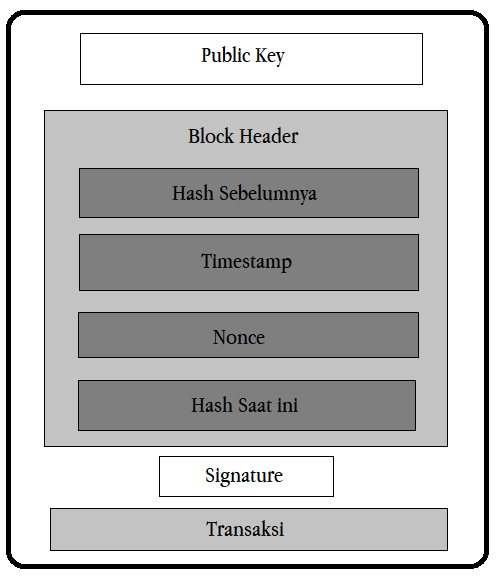
\includegraphics[scale=0.6]{gambar/isi-blok.png}
  \caption{Ilustrasi isi blok}
  \label{fig:isiblok}
\end{figure}

Dari blok yang dibuat, dapat dilihat dari ilustrasi gambar di atas ada beberapa bagian dari suatu blok.Ilustrasi ini merupakan ilustrasi penyederhanaan isi dari suatu blok dari Ethereum. Dalam suatu blok terkandung beberapa bagian yaitu public key, block header, transaksi, dan digital signature. Public key adalah sebuah serangkaian hash yang digunakan sebagai autentikasi data dari transaksi Ethereum. Kemudian ada block header sebagai inti dari sebuah blok dari blockchain yang berisi hash saat ini, kapan transaksi dilakukan dan durasi transaksi, hash sebelumnya, nonce, hingga jenis transaksi yang dilakukan. Semua dapat terlihat pada gambar berikut.

\begin{figure}[htp]
\centering
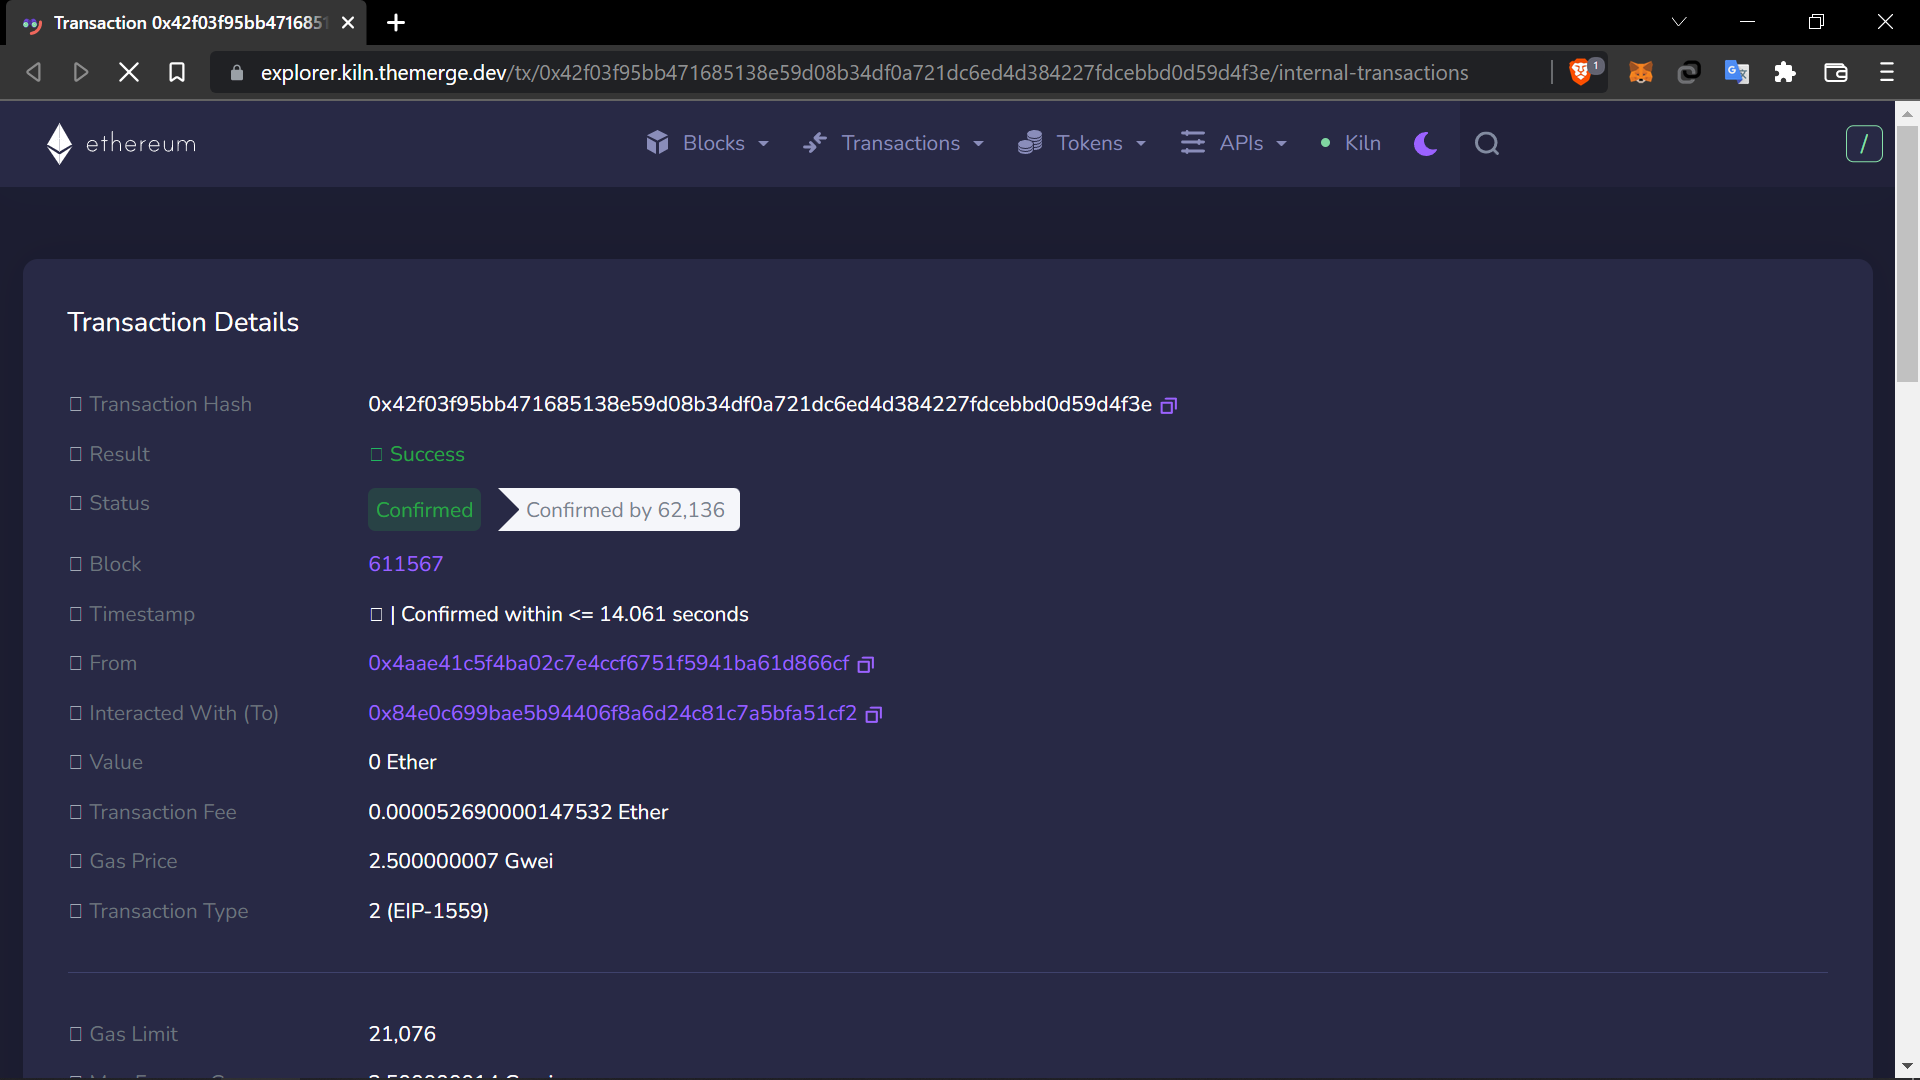
\includegraphics[scale=0.2]{gambar/isi-blok-2.png}
\caption{Gambar isi suatu blok dari blockchain} 
\label{fig:isiblok2}
\end{figure}

Kemudian, dalam blok juga terdapat signature yang dilakukan. Signature ini adalah sebagaian hash yang ditambahkan di dalam hash saat ini yang menandakan jenis yang memvalidasi transaksi yang dilakukan. Seperti pada contoh gambar dibawah terdapat Hex 0x2000 yang merupakan tanda transaksi dilakukan dari Smart Contract yang dibuat. Terakhir, transaksi yang telah dilakukan perincian jumlah gas yang dipakai, harga gas, nonce, hingga harga yang dibayarkan. Berikut isi dalam blok Ethereum.

\begin{figure}[htp]
\centering
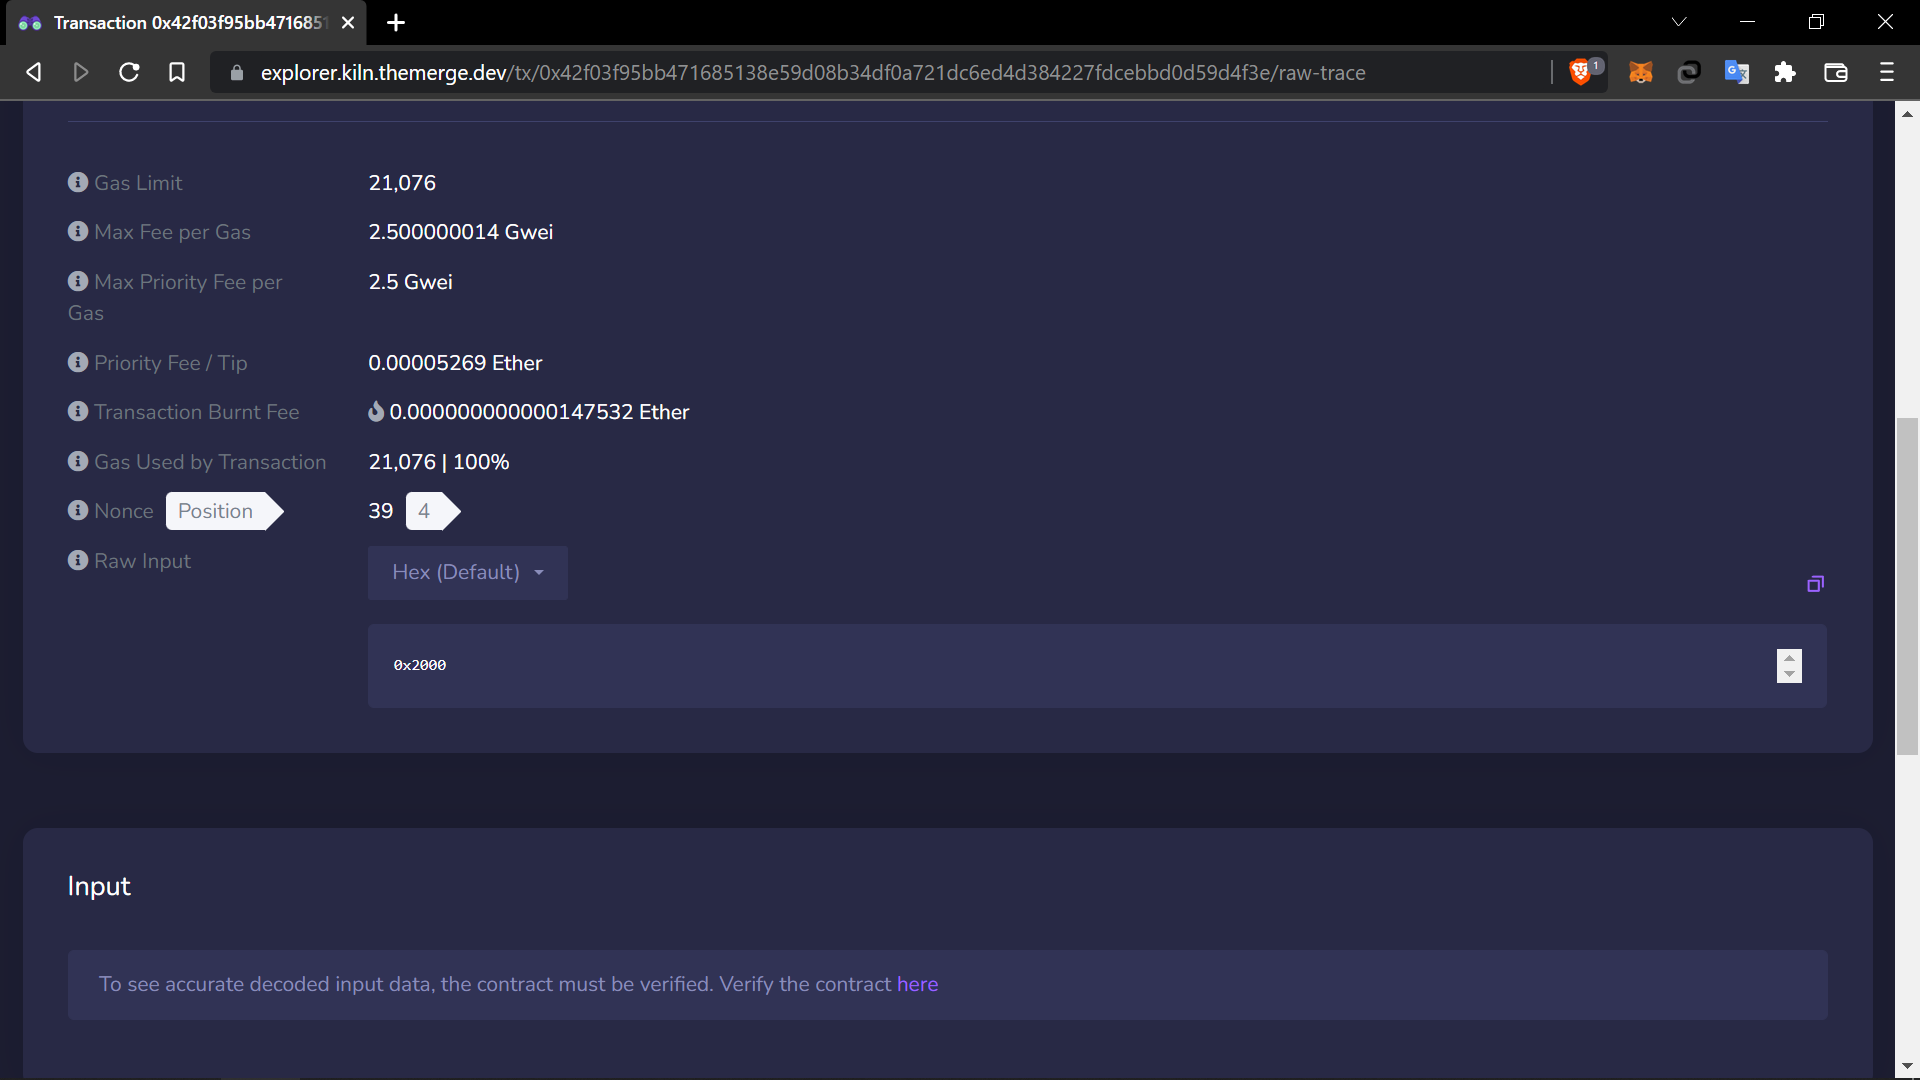
\includegraphics[scale=0.2]{gambar/isi-blok-3.png}
\caption{Isi dari Blok}
\label{fig:isiblok3}
\end{figure}

\subsection{Decentralized Applications}
\label{subsec:dapps}

\begin{figure}[htp!]
\centering
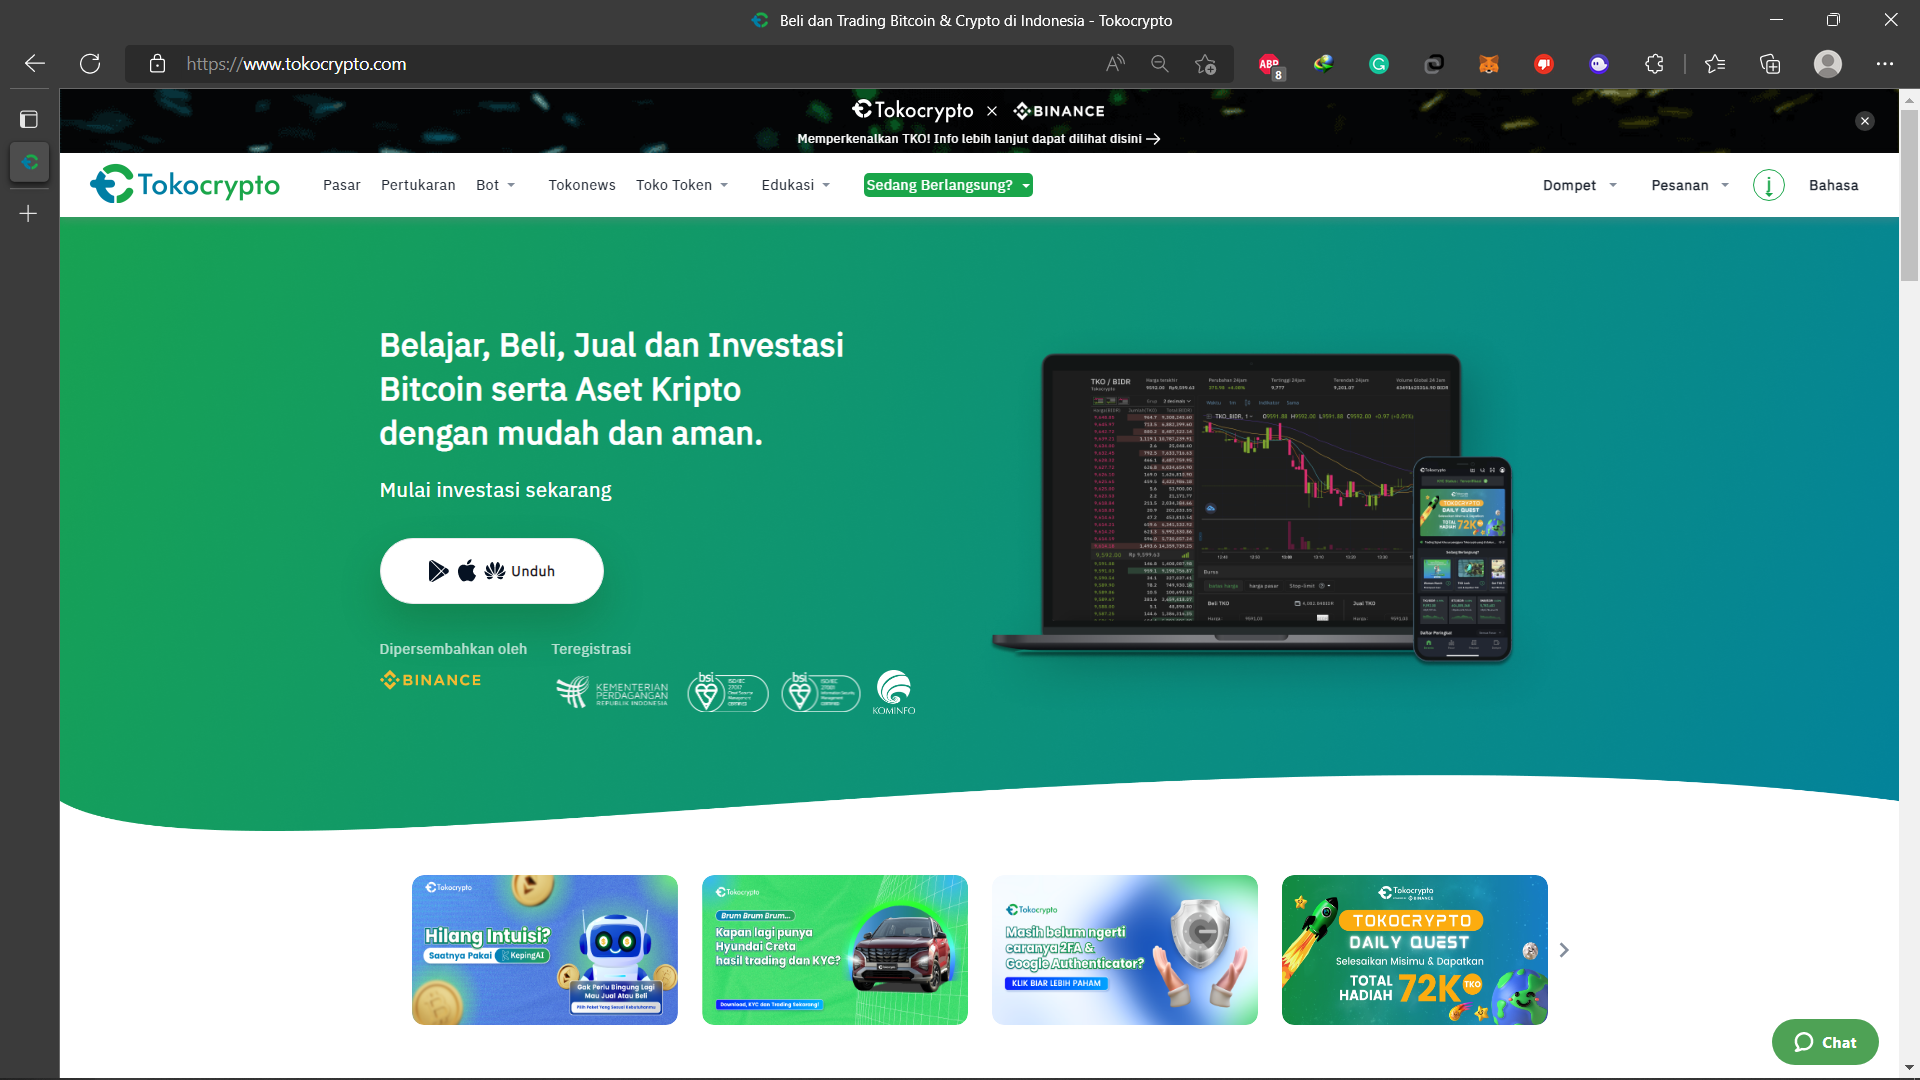
\includegraphics[scale=0.2]{gambar/tokocrypto.png}
\caption{Contoh salah satu Decentralized App di Indonesia, yaitu Tokocrypto : Exchanger Crypto di Indonesia}
\label{fig:tokocrypto}
\end{figure}

Decentralized applications adalah sebuah konsep aplikasi berbasis yang terintegrasi dengan blockchain. Decentralized ini adalah sebuah peleburan antara web 2.0 dengan web 3.0. Peleburan aplikasi ini dimaksudkan sebagai aplikasi yang bisa menyokong Decentralized app ini terdiri atas beberapa bagian yaitu backend, frontend, data storage, hingga protokol komunikasi \cite{MasteringEthGavinWood}. Untuk bisa disebut sebagai decentralized apps, sebuah aplikasi harus memenuhi ketiga aspek:

\begin{itemize}
\item{Ketahanan}
\\ Ketahanan dalam mengelola pelbagai transaksi dalam satu waktu, maka dari itu decentralized apps perlu kemampuan bertahan dalam kondisi menjalankan pelbagai transaksi meski dengan perawatan sistem yang tidak menentu.
\item{Transparan}
\\ Dalam keadaan default, suatu blockchain harus memberikan transparansi kepada seluruh penggunanya. Segala seluk beluk aplikasi mulai dari source code, kerjasama,hingga segala persetujuan bisa dilihat dan diaudit oleh semua pengguna. Dan segala bentuk perubahan harus disimpan di blockchain itu sendiri.
\item{Censorship Resistance}
\\ Pengguna harus mampu mengoperasikan decentralized app dalam secara langsung tanpa ada tokoh penengan tersentral. Artinya dalam pengoperasiannya pengguna harus mampu mengakses decentralized app melalui suatu node dengan mudah.
\end{itemize}

\subsection{\emph{Proof of Stake}}
\label{subsec:pos}

\emph{Proof of Stake} atau PoS adalah sebuah konsensus yang mengambil keputusan berdasarkan sejumlah pertaruhan sebuah pengguna yang terdaftar di dalam jaringan \emph{Blockchain}. Dalam praktiknya PoS tidak memanfaatkan kemampuan komputer pengguna yang terhubung dengan jaringan melainkan memanfaatkan seberapa banyak \emph{cryptocurrencies} yang dia miliki di dalam jaringan tersebut. Banyaknya \emph{cryptocurrencies} yang pengguna miliki akan memengaruhi proses konsensus yang terjadi di jaringan tersebut dan meningkatkan probabilitas pengguna tersebut untuk dipilih untuk berpartisipasi untuk membuat blok dari rangkaian blok yang sedang dibuat \cite{poscons}. Diatas kertas PoS memiliki beberapa keunggulan tersendiri. Dikarenakan tidak menggunakan komputer yang pengguna gunakan, maka PoS tidak memerlukan energi yang besar untuk menjalankan proses pembuatan blok. Kemudian dikarenakan tidak menggunakan energi yang besar otomatis waktu yang dibutuhkan untuk melakukan pembuatan blok pun tidak membutuhkan waktu banyak. Serangkaian kegiatan yang dilakukan oleh PoW seperti memecahkan kriptografi tidak perlu dilakukan dengan waktu yang lama. PoS banyak digunakan di beberapa \emph{blockchain} yang ada seperti Cardano, Solana, hingga Ethereum 2.0.
\\
\emph{Proof of Stake} sendiri dikarenakan menggantikan sebuah konsesus yang telah ada ditargetkan PoS akan memiliki implementasi yang lebih baik dari PoW. Pertama bisa digunakan dalam perangkat \emph{low-power} yang biasa ditemui di masyarakat seperti IoT. Terlebih PoS akan meningkatkan kesempatan perangkat yang terhubung untuk berinteraksi tanpa konsumsi energi yang tinggi. \emph{Proof of Stake} juga mempunyai keunggulan yang tidak dimiliki \emph{Proof of Work} yaitu kemudahan. Tentu kemudahan yang dimaksud yaitu kemudahan dalam setup dan validasi menggunakan perangkat di jaringan \emph{Blockchain} berbasis \emph{Proof of Stake}. Dengan menggunakan \emph{Proof of Stake} pengguna maupun validator tidak memerlukan banyak bahan untuk melakukan persiapan dan ikut dalam jaringan ini. 

\section{\emph{Ethereum}}
\label{sec:eth}

\emph{Ethereum} adalah sebuah blockchain yang menggunakan konsendus \emph{Proof of Stake} untuk membuat blok. Pada sistem Ethereum, sistem ini bersifat open-source dan terdesentralisasi. Dibuat pertama kali pada tahun 2013 oleh Vitalik Buterin, awalnya dibuat sebagai sistem mesin berbasis transaksi yang mana dalam inisiasi sistem terdapat blok pertama dari sebuah blockchain yang berisi instruksi awal dari seluruh sistem mulai dari konsensus, cara pembuatan blok, limit gas, harga gas, hingga alamat awal (yang biasa disebut sebagai blok genesis) kemudian blok utama ini melakukan segala perintah dari blok genesis kemudian melakukannya berulang kali di seluruh mesin yang terhubung ke dalam sistem ini \cite{MasteringEthGavinWood}. Ethereum dibuat sebagai kompetitor dari Bitcoin yang telah diluncurkan dari tahun 2009 bukan hanya sekedar pengganti uang fisik, namun sebagai sebuah sistem terorganisir yang bisa saling berinteraksi dan beririsan antara satu bisnis dengan bisnis lainnya. Ethereum sebagai blockchain yang bersaing langsung dengan Bitcoin sendiri punya beberapa keunggulan dibandingkan dengan Bitcoin. Berikut adalah perbedaan Ethereum dengan Bitcoin secara umum:

\begin{longtable}{|p{4cm}|p{5cm}|p{5cm}|}
  \caption{Tabel Perbandingan \emph{Ethereum} dan \emph{Bitcoin} sebagai sistem Blockchain}
  \label{tb:ethvsbitcoin}\\
  \hline
  \rowcolor[HTML]{C0C0C0}
  \textbf{Aspek} & \textbf{Ethereum} & \textbf{Bitcoin} \\
  \hline
Tahun Peluncuran & 2009 & 2015 \\
  \hline
Konsensus yang digunakan & Proof of Work dan Proof of Stake & Proof of Stake \\
  \hline
Waktu pembuatan blok & ~10 menit & 10-15 detik \\
  \hline
Jumlah suplai & 21 juta & tidak terbatas \\
  \hline
Perkiraan kemampuan transaksi per detik & 7 & 30 \\
 \hline
\end{longtable}

Pada awal perilisan,Ethereum menggunakan PoW untuk melakukan segala proses pembuatan blok dan \emph{scalability}. Karena hal tersebut pada perkembangan awal jaringan ini sangat memerlukan komputer yang mampu untuk melakukan segala proses yang terjadi. Mulai dari memilik pengguna, membuat blok, hingga pengiriman blok memerlukan komputer yang mampu. Dalam satu sisi PoW ini bermanfaat karena pada awal jaringan memerlukan konsensus yang sederhana tidak memerlukan banyak pemrograman. Selain itu PoW juga membuat sistem objektif dalam memilih pengguna untuk membuat blok. Kemungkinan untuk didominasi lebih kecil karena apabila akan melakukan dominasi, perlu banyak hardware yang dikorbankan dan energi yang dikonsumsi sangat besar bahkan memerlukan jaringan energi khusus \cite{poscons}. Karena hal ini Ethereum melakukan proses migrasi menuju konsensus yang lebih hemat energi yaitu PoS. PoS bermaksud untuk mengurangi konsumsi energi secara derastis dan meningkatkan \emph{scalability} yang lebih baik.

\subsection{Ethereum Virtual Machine}
\label{subsec:evm}

Ethereum Virtual Machine adalah sebuah bagian dari Ethereum yang merupakan tempat melakukan interaksi dan deploy Smart Contract \cite{MasteringEthGavinWood}. EVM adalah komputer tempat melakukan berbagai kegiatan dan pelaksanaan transaksi Smart Contract. EVM pada sistem Etherum sendiri merupakan tempat eksekusi program berbahasa Solidity. EVM dapat memilah apa saja yang bisa dilakukan dengan EVM dan apa saja yang tidak bisa dilakukan dengan EVM. EVM mempunyai arsitektur seperti berikut :
\\
\begin{figure}[htp]
\centering
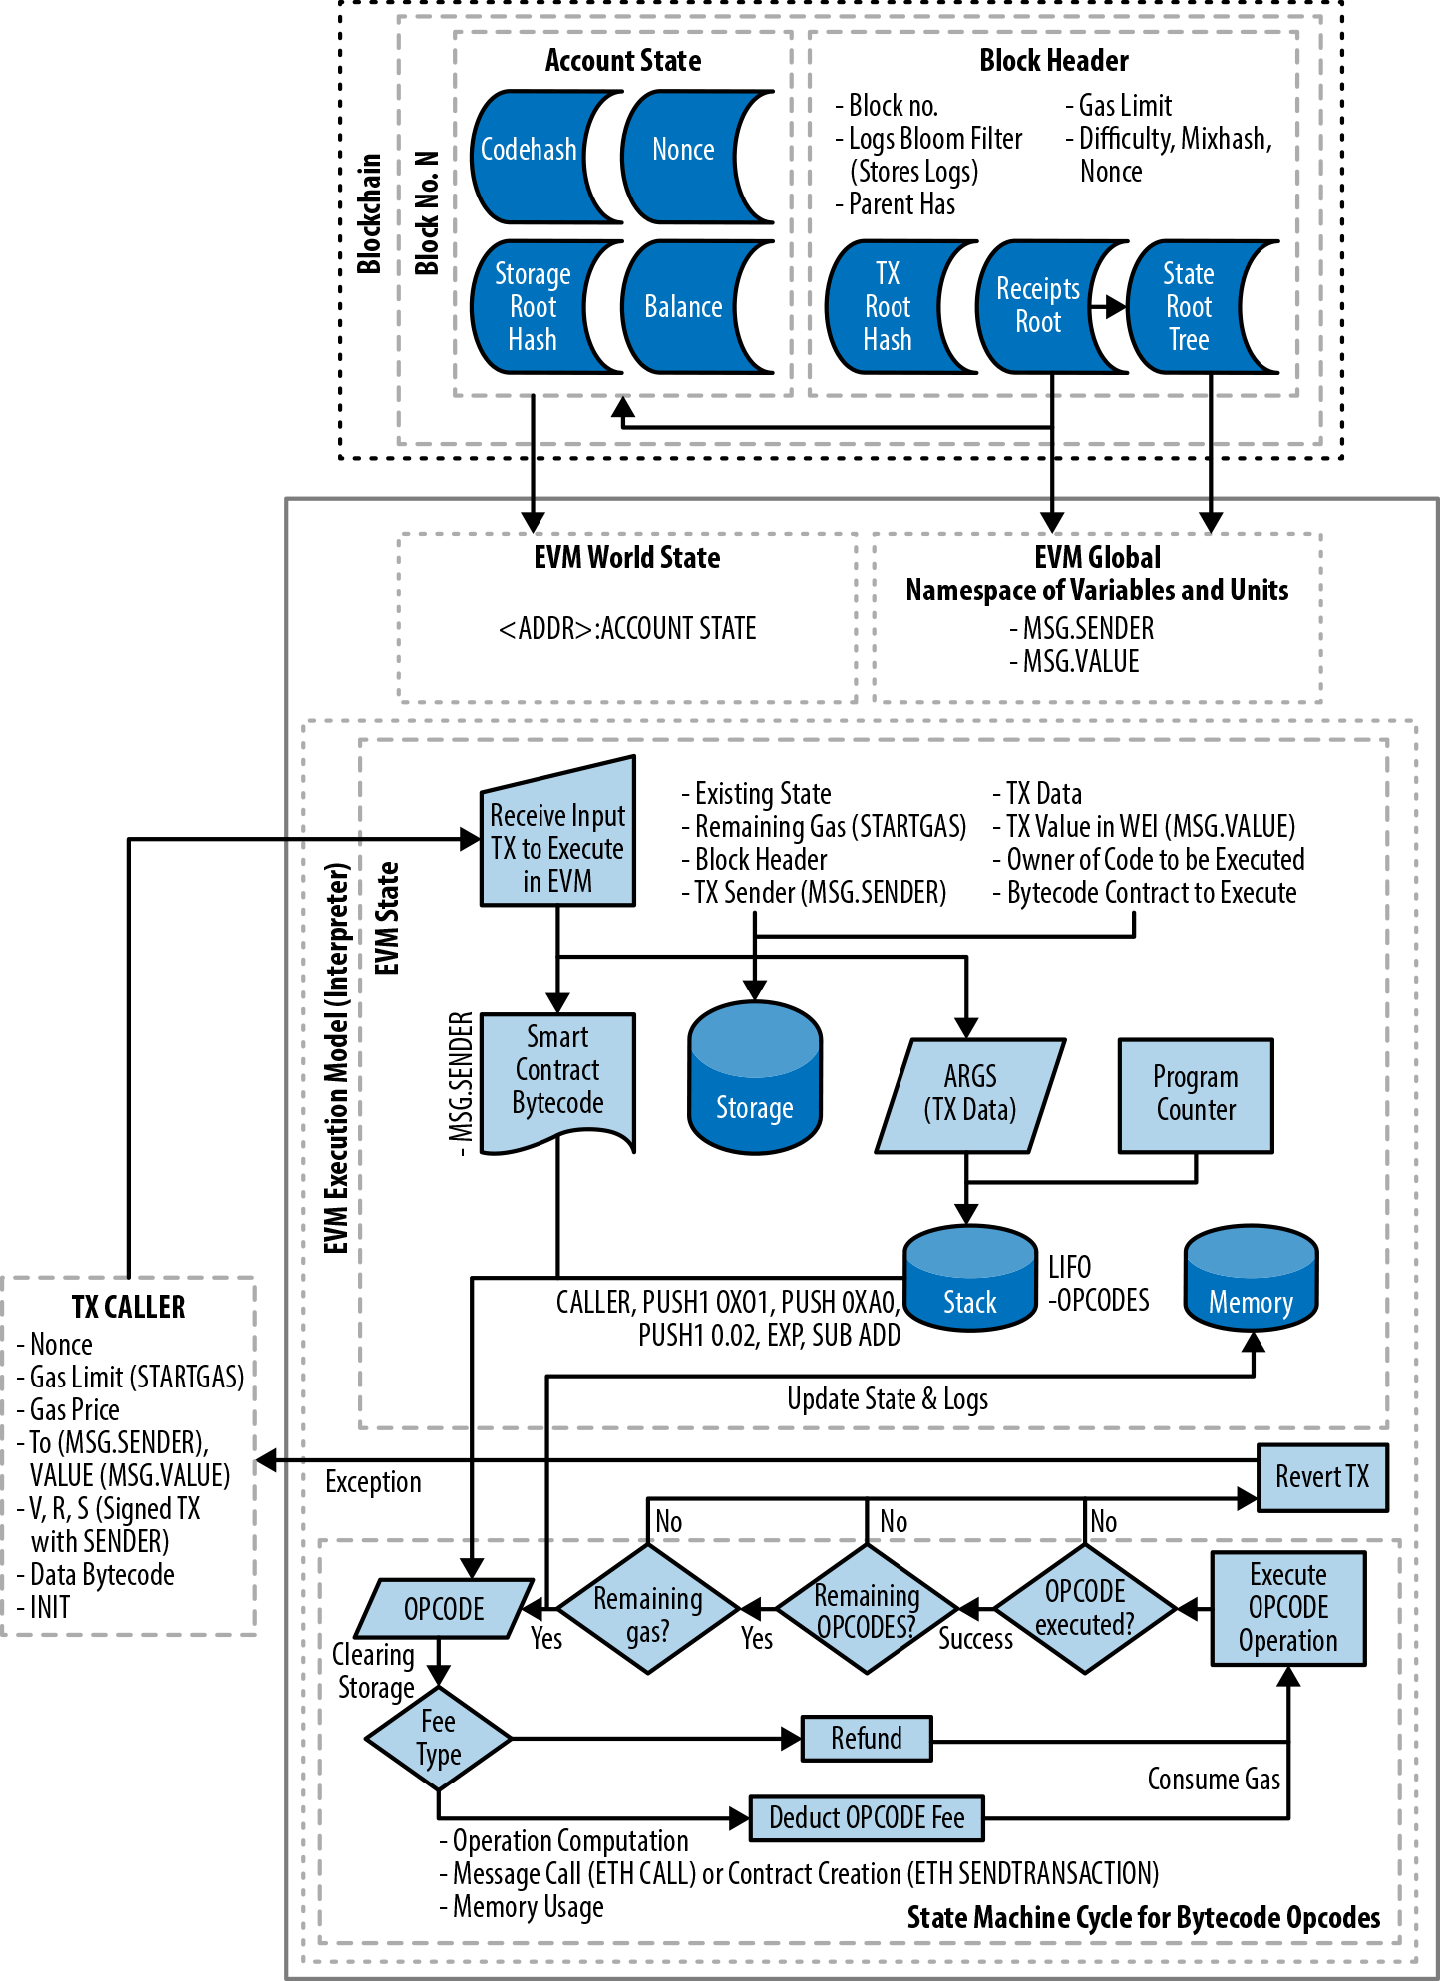
\includegraphics[scale=1.2]{gambar/arsitektur-evm.png}
\caption{Arsitektur EVM}
\end{figure}

Pada gambar arsitektur, dapat dilihat EVM memilah dan menjalankan program sesuai dengan ketersediaan gas yang diberikan dari akun yang melakukan request transaksi. Seperti yang telah dijelaskan pada 2.4.1, gas diperlukan sebagai biaya utama untuk diberikan ke pada EVM untuk melakukan proses deploy dan interaksi Smart Contract. Gas ini digunakan di dalam EVM untuk mengeksekusi program dengan harga variatif. Berikut harga untuk beberapa operasi aritmatika maupun kompleks:
\begin{itemize}
\item{Penambahan dan Pengurangan}\\Untuk operasi ini bernilai 3 gas unit
\item{Perkalian dan Pembagian}\\Untuk operasi ini bernilai 5 gas unit
\item{Logic operation}\\Untuk operasi ini bernilai 3 gas unit
\item{Hashing}\\Untuk operasi SHA3 hash bernilai (30 + 6*(\emph{n})) gas unit dengan \emph{n} untuk setiap 256 bit data yang telah melalui operasi hash
\item{Mengirim transaksi}\\Untuk mengirimkan transaksi bernilai 21000 gas unit
\item{Mengecek saldo}\\Untuk mengecek saldo bernilai 400 gas unit
\item{Info umum}\\Untuk mengecek address, caller, dan timestamp bernilai 2 gas unit
\item{Membuat blok}\\Untuk membuat blok bernilai 32000 gas unit
\item{Memanggil fungsi}\\Untuk memanggil fungsi bernilai mulai dari 700 gas unit
\item{Pembukaan akun}\\Untuk membuat akun diperlukan bernilai 30000 gas unit dan untuk menghapus atau mengedit akun bernilai 5000 gas unit 
\end{itemize}
Karena EVM melakukan perhitungan sebagai \emph{stack machine} dengan nilai satu blok memori sebesar 256 bit. EVM mempunyai beberapa instruksi set yaitu:
\begin{itemize}
\item{Aritmatika dan Logic Operations}
\item{Logging}
\item{Control Flow}
\item{Stack, Memory, dan akses penyimpanan}
\item{Pencarian kode}
\end{itemize}

\subsection{Perbedaan \emph{Proof of Stake} dan \emph{Proof of Work}}
\label{subsec:powandposdiffer}

Dalam proses seleksi siapa yang berhak untuk menjadi validator dalam suatu transaksi \emph{Ethereum}, terdapat beberapa kesepakatan bersama/konsensus yang digunakan dalam memilih validator. Saat ini terdapat dua konsensus yang umum digunakan berbagai macam \emph{Cryptocurrencies} yaitu \emph{Proof of Stake} dan \emph{Proof of Work} \cite{9388487}. Berikut adalah perbandingan antara keduanya.

\begin{longtable}{|p{4cm}|p{5cm}|p{5cm}|}
  \caption{Tabel Perbandingan \emph{Proof of Stake} dan \emph{Proof of Work}}
  \label{tb:posandpowdifference}\\
  \hline
  \rowcolor[HTML]{C0C0C0}
  \textbf{Ciri} & \textbf{Proof of Stake} & \textbf{Proof of Work} \\
  \hline
Cara membuat blok & Melakukan validasi pengirim dan penerima dengan mencocokkan kunci publik antara satu dengan lainnya & Melakukan pemecahan soal matematika kompleks untuk melakukan suatu transaksi \\
  \hline
  Memilih validator & Berdasarkan jumlah \emph{cryptocurrencies} yang dipegang satu akun & Berdasarkan raw power komputer yang dipegang satu akun \\
  \hline
  Konsumsi daya & Rendah karena tidak memerlukan raw power komputer & Tinggi karena memanfaatkan semua raw power yang diberikan \\
 \hline
 Ketahanan sistem & Sistem tidak terlalu baik karena validator stagnan dan mengonsumsi daya tahan penyimpanan lokal & Sistem cukup baik karena validator selalu meningkatkan raw power komputer. Otomatis perangkat diperbarui secara berkala\\
 \hline
Kecepatan pembuatan blok & Lebih cepat karena tidak perlu raw power komputer & Lebih lambat karena perlu raw power komputer\\
\hline
  Skalabilitas & Cukup baik dalam meningkatkan jumlah transaksi dalam satu interval & Cukup baik dalam meningkatkan jumlah transaksi dalam satu interval\\
\hline 
\end{longtable}